\section{\RU{Многомерные массивы}\EN{Multidimensional arrays}}

\RU{Внутри, многомерный массив выглядит так же, как и линейный.}
\EN{Internally, a multidimensional array is essentially the same thing as a linear array.}

\RU{Ведь память компьютера линейная, это одномерный массив.
Но для удобства, этот одномерный массив легко представить как многомерный.}
\EN{Since the computer memory is linear, it is an one-dimensional array.
For convenience, this multi-dimensional array can be easily represented as one-dimensional.}

\RU{К примеру, вот как элементы массива $a[3][4]$ расположены в одномерном массиве из 12-и ячеек:}
\EN{For example, thit is how the elements of the $a[3][4]$ array are placed in one-dimensional array of 12 cells:}

\begin{table}[H]
\centering
\begin{tabular}{ | l | }
\hline
[0][0] \\
\hline
[0][1] \\
\hline
[0][2] \\
\hline
[0][3] \\
\hline
[1][0] \\
\hline
[1][1] \\
\hline
[1][2] \\
\hline
[1][3] \\
\hline
[2][0] \\
\hline
[2][1] \\
\hline
[2][2] \\
\hline
[2][3] \\
\hline
\end{tabular}
\caption{\RU{Двухмерный массив представляется в памяти как одномерный}
\EN{Two-dimensional array represented in memory as one-dimensional}}
\end{table}

\RU{Вот по каким адресам в памяти располагается каждая ячейка двухмерного массива 3*4:}
\EN{Here is how each cell of 3*4 array are placed in memory:}

\begin{table}[H]
\centering
\begin{tabular}{ | l | l | l | l | }
\hline                        
0 & 1 & 2 & 3 \\
\hline  
4 & 5 & 6 & 7 \\
\hline  
8 & 9 & 10 & 11 \\
\hline  
\end{tabular}
\caption{\RU{Адреса в памяти каждой ячейки двухмерного массива}
\EN{Memory addresses of each cell of two-dimensional array}}
\end{table}

\index{row-major order}
\RU{То есть, чтобы вычислить адрес нужного элемента, в начале умножаем первый индекс на 4 (ширину матрицы), 
затем прибавляем второй индекс.}
\EN{So, in order to calculate the address of the element we need, we first multiply the first index by
4 (matrix width) and then add the second index.}
\RU{Это называется}\EN{That's called} \IT{row-major order}, 
\RU{и такой способ представления массивов и матриц используется по крайней мере в}
\EN{and this method of array and matrix representation is used in at least} \CCpp \AndENRU Python. 
\EN{The term}\RU{Термин} \IT{row-major order} \RU{означает по-русски
примерно следующее: \q{в начале записываем элементы первой строки, затем второй \dots и элементы последней 
строки в самом конце}.}
\EN{in plain English language means: \q{first, write the elements of the first row, then the second row \dots 
and finally the elements of the last row}.}

\index{column-major order}
\index{FORTRAN}
\RU{Другой способ представления называется}\EN{Another method for representation is called} 
\IT{column-major order} 
(\RU{индексы массива используются в обратном порядке}\EN{the array indices are used in reverse order}) 
\RU{и это используется по крайней мере в}\EN{and it is used at least in} FORTRAN, MATLAB \AndENRU R. 
\RU{Термин }\IT{column-major order} \RU{означает по-русски
следующее: \q{в начале записываем элементы первого столбца, затем второго \dots и элементы последнего столбца
в самом конце}.}
\EN{term in plain English language means: \q{first, write the elements of the first column, then the second column \dots
and finally the elements of the last column}.}

\RU{Какой из способов лучше}\EN{Which method is better}?
\RU{Вообще, в терминах производительности и кэш-памяти, лучший метод организации данных это тот,
при котором к данным обращаются последовательно.}
\EN{In general, in terms of performance and cache memory, 
the best scheme for data organization is the one,
in which the elements are accessed sequentially.}
\RU{Так что если ваша функция обращается к данным построчно, то \IT{row-major order} лучше,
и наоборот.}
\EN{So if your function accesses data per row, \IT{row-major order} is better, and vice versa.}

% subsections
\subsection{\RU{Пример с двумерным массивов}\EN{Two-dimensional array example}}

\EN{We will work with array of \Tchar type, meaning that each element require only one 
byte in memory.}
\RU{Мы будем работать с массивом типа \Tchar, это значит, что каждый элемент требует
только одного байта в памяти.}

\subsubsection{\RU{Пример с заполнением строки}\EN{Row filling example}}
\index{\olly}

\RU{Заполняем вторую строку значениями}\EN{Let's fill the second row with values:} $0 \ldots 3$:

\lstinputlisting[caption=\RU{Пример с заполнением строки}\EN{Row filling example}]{patterns/13_arrays/5_multidimensional/two1.c.\LANG}

\RU{Я обвел красным все три строки}\EN{I marked all three rows with red}. 
\RU{Видно что во второй теперь имеются байты}\EN{We see that second row now has values} 
0, 1, 2 \AndENRU 3:

\begin{figure}[H]
\centering
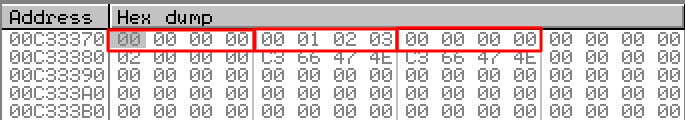
\includegraphics[scale=\NormalScale]{patterns/13_arrays/5_multidimensional/olly_2D_1.png}
\caption{\olly: \RU{массив заполнен}\EN{array is filled}}
\end{figure}

\subsubsection{\RU{Пример с заполнением столбца}\EN{Column filling example}}
\index{\olly}

\RU{Заполняем третий столбец значениями}\EN{Let's fill the third column with values:} $0 \ldots 2$.

\lstinputlisting[caption=\RU{Пример с заполнением столбца}\EN{Column filling example}]{patterns/13_arrays/5_multidimensional/two2.c.\LANG}

\RU{Здесь я также обвел красным три строки}\EN{I also marked three rows by red here}. 
\RU{Видно что в каждой строке, на третьей позиции, теперь записаны}
\EN{We see that in each row, at third position, these values are written:} 0, 1 \AndENRU 2.

\begin{figure}[H]
\centering
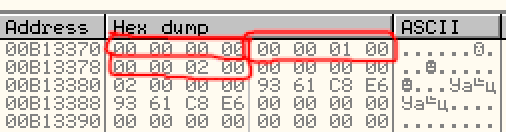
\includegraphics[scale=\NormalScale]{patterns/13_arrays/5_multidimensional/olly_2D_2.png}
\caption{\olly: \RU{массив заполнен}\EN{array is filled}}
\end{figure}

\subsection{\RU{Работа с двухмерным массивом как с одномерным}
\EN{Access two-dimensional array as one-dimensional}}

\RU{Мы можем легко убедиться, что можно работать с двухмерным массивом как с одномерным,
используя по крайней мере два метода:}
\EN{We can be easily assured that it's possible to access a two-dimensional array as one-dimensional array in at least two ways:}

\lstinputlisting{patterns/13_arrays/5_multidimensional/2D_as_1D.c.\LANG}

\RU{Компилируете и запускаете: мы увидим корректные значения.}
\EN{Compile and run it: it shows correct values.}

\RU{Очарователен результат работы MSVC 2013~--- все три процедуры одинаковые!}
\EN{What MSVC 2013 did is fascinating, all three routines are just the same!}

\lstinputlisting[caption=\Optimizing MSVC 2013 x64]{patterns/13_arrays/5_multidimensional/2D_as_1D_MSVC_2013_Ox_x64.asm.\LANG}

\RU{GCC сгенерировал практически одинаковые процедуры:}
\EN{GCC also generates equivalent routines, but slightly different:}

\lstinputlisting[caption=\Optimizing GCC 4.9 x64]{patterns/13_arrays/5_multidimensional/2D_as_1D_GCC49_x64_O3.s.\LANG}

\subsection{\RU{Пример с трехмерным массивом}\EN{Threedimensional array example}}

\RU{То же самое и для многомерных массивов.}\EN{Same thing about multidimensional arrays.}

\RU{На этот раз будем работать с массивом типа \Tint: каждый элемент требует 4 байта в памяти.}
\EN{Now we will work with array of \Tint type: each element require 4 bytes in memory.}

\RU{Попробуем}\EN{Let's see}:

\lstinputlisting[caption=\RU{простой пример}\EN{simple example}]{patterns/13_arrays/5_multidimensional/multi.c}

\subsubsection{x86}

\RU{В итоге}\EN{We got} (MSVC 2010):

\lstinputlisting[caption=MSVC 2010]{patterns/13_arrays/5_multidimensional/multi_msvc.asm}

\RU{В принципе, ничего удивительного. В \TT{insert()} для вычисления адреса нужного элемента массива, 
три входных аргумента перемножаются по формуле $address=600 \cdot 4 \cdot x + 30 \cdot 4 \cdot y + 4z$, 
чтобы представить массив трехмерным.
Не забывайте также, что тип \Tint 32-битный (4 байта), поэтому все коэффициенты нужно умножить на 4.}
\EN{Nothing special. For index calculation, three input arguments are multiplying 
by formula $address=600 \cdot 4 \cdot x + 30 \cdot 4 \cdot y + 4z$ to represent array as multidimensional.
Do not forget the \Tint type is 32-bit (4 bytes),
so all coefficients must be multiplied by 4.}

\lstinputlisting[caption=GCC 4.4.1]{patterns/13_arrays/5_multidimensional/multi_gcc.asm}

\RU{Компилятор GCC решил всё сделать немного иначе}\EN{GCC compiler does it differently}.
\RU{Для вычисления одной из операций ($30y$), GCC создал код, где нет самой операции умножения.}
\EN{For one of operations calculating ($30y$), GCC produced a code without multiplication instruction.}
\RU{Происходит это так}\EN{This is how it done}: 
$(y+y) \ll 4 - (y+y) = (2y) \ll 4 - 2y = 2 \cdot 16 \cdot y - 2y = 32y - 2y = 30y$. 
\RU{Таким образом, для вычисления $30y$ используется только операция сложения, 
операция битового сдвига и операция вычитания.}\EN{Thus, for $30y$ calculation, only one addition operation
used, one bitwise shift operation and one subtraction operation.}
\RU{Это работает быстрее}\EN{That works faster}.

\subsubsection{ARM + \NonOptimizingXcodeIV (\ThumbMode)}

\lstinputlisting[caption=\NonOptimizingXcodeIV (\ThumbMode)]{patterns/13_arrays/5_multidimensional/multi_Xcode_thumb_O0_\LANG.asm}

\NonOptimizing LLVM \RU{сохраняет все переменные в локальном стеке, хотя это и избыточно.}
\EN{saves all variables in local stack, however, it is redundant.}
\RU{Адрес элемента массива вычисляется по уже рассмотренной формуле.}
\EN{Address of array element is calculated by formula we already figured out.}

\subsubsection{ARM + \OptimizingXcodeIV (\ThumbMode)}

\lstinputlisting[caption=\OptimizingXcodeIV (\ThumbMode)]{patterns/13_arrays/5_multidimensional/multi_Xcode_thumb_O3_\LANG.asm}

\RU{Тут используются уже описанные трюки для замены умножения на операции сдвига, сложения и вычитания.}
\EN{Here is used tricks for replacing multiplication by shift, addition and subtraction we already considered.}

\index{ARM!\Instructions!RSB}
\index{ARM!\Instructions!SUB}
\RU{Также мы видим новую для себя инструкцию}\EN{Here we also see new instruction for us:} 
\TT{RSB} (\IT{Reverse Subtract}).
\RU{Она работает так же, как и \SUB, только меняет операнды местами.}
\EN{It works just as \SUB, but swapping operands with each other.}
\RU{Зачем?}\EN{Why?}
\index{ARM!Optional operators!LSL}
\SUB, \TT{RSB}, \RU{это те инструкции, ко второму операнду которых можно применить коэффициент сдвига, 
как мы видим и здесь}
\EN{are those instructions, to the second operand of which shift coefficient may be applied}: (\TT{LSL\#4}). 
\RU{Но этот коэффициент можно применить только ко второму операнду.}
\EN{But this coefficient may be applied only to second operand.}
\RU{Для коммутативных операций, таких как сложение или умножение, 
там операнды можно менять местами и это не влияет на результат.}
\EN{That's fine for commutative operations like addition or multiplication, operands may be swapped there
without result affecting.}
\RU{Но вычитание ~--- операция некоммутативная, так что, для этих случаев существует инструкция \TT{RSB}.}
\EN{But subtraction is non-commutative operation, so, for these cases, \TT{RSB} exist.}

\index{ARM!\Instructions!LDR.W}
\RU{Инструкция }\TT{``LDR.W R9, [R9]''} \RU{работает как}\EN{instruction works like} \LEA~(\ref{sec:LEA})
\RU{в x86, и здесь она ничего не делает, она избыточна.}\EN{in x86, but here it does nothing, it is redundant.}
\RU{Вероятно, компилятор несоптимизировал её.}\EN{Apparently, compiler not optimized it.}



\ifx\LITE\undefined
\subsection{\RU{Еще примеры}\EN{More examples}}

\RU{Компьютерный экран представляет собой двухмерный массив, но видеобуфер это линейный
одномерный массив}\EN{The computer screen is represented as a 2D array, but the video-buffer is 
a linear 1D array}. 
\RU{Мы рассматриваем это здесь}\EN{We talk about it here}: \myref{Mandelbrot_demo}.
\fi
